\documentclass{article}
\usepackage{amsmath, amssymb, amsthm, graphicx}
\title{Area of a regular polygon}
\author{Andrew Taylor}
\date{August 4 2022}
\begin{document}
\maketitle

\begin{figure}[h]
\centering
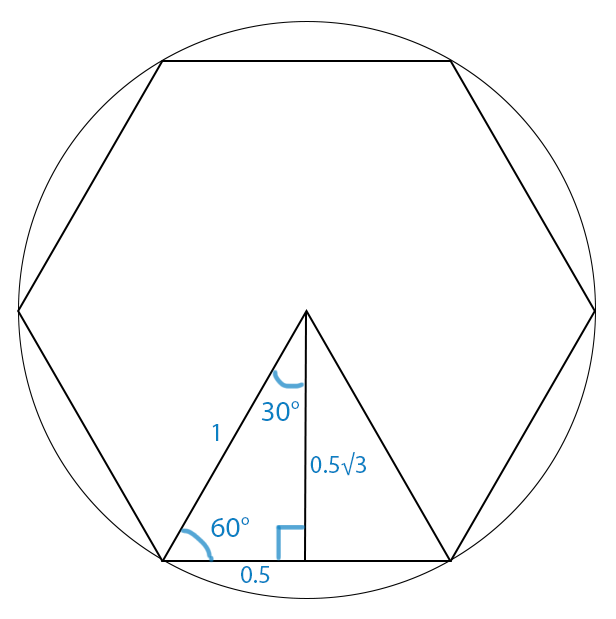
\includegraphics[width=7cm]{regularhexagoninscribed}
\end{figure}

In the figure above, the area of the equilateral triangle is given by:
\begin{align*}
A_{T} &= \dfrac{1}{2}bh \\
&= \dfrac{1}{2}\left(2\sin\dfrac{\pi}{6}\right)\left(\cos\dfrac{\pi}{6}\right) \\
&= \sin\dfrac{\pi}{6}\cos\dfrac{\pi}{6} \\
\end{align*}

The area of the regular hexagon is six times the area of the triangle.
\begin{align*}
A_{H} &= 6A_{T} \\
&= 6\sin\dfrac{\pi}{6}\cos\dfrac{\pi}{6} \\
&=\dfrac{3\sqrt{3}}{2}
\end{align*}

This formula generalizes for a regular n-sided polygon. The area of a regular n-sided polygon inscribed in a unit circle is given by:

\begin{equation}
A_{P} = n \sin \dfrac{\pi}{n} \cos \dfrac{\pi}{n}
\end{equation}

As n approaches infinity, the area of the polygon approaches $\pi$.

\begin{equation}
\lim_{n \to \infty} \left( n \sin \dfrac{\pi}{n} \cos \dfrac{\pi}{n} \right) = \pi
\end{equation}

When the circle has radius r, we get the equations:

\begin{equation}
A_{P} = \left( n \sin \dfrac{\pi}{n} \cos \dfrac{\pi}{n} \right) r^2
\end{equation}

\begin{equation}
\lim_{n \to \infty} \left( n \sin \dfrac{\pi}{n} \cos \dfrac{\pi}{n} \right) r^2 = \pi r^2
\end{equation}

These equations give us an approximation of $\pi$. For example:
\begin{align*}
A_{10} &= 10 \sin \dfrac{\pi}{10} \cos \dfrac{\pi}{10} &= 2.93892626146236546347 \\
A_{100} &= 10^2 \sin \dfrac{\pi}{10^2} \cos \dfrac{\pi}{10^2} &= 3.13952597646566866629 \\
A_{1000} &= 10^3 \sin \dfrac{\pi}{10^3} \cos \dfrac{\pi}{10^3} &= 3.14157198277947591336 \\
A_{10,000} &= 10^4 \sin \dfrac{\pi}{10^4} \cos \dfrac{\pi}{10^4} &= 3.14159244688128591605 \\
A_{100,000} &= 10^5 \sin \dfrac{\pi}{10^5} \cos \dfrac{\pi}{10^5} &= 3.14159265152270750221 \\
A_{1,000,000} &= 10^6 \sin \dfrac{\pi}{10^6} \cos \dfrac{\pi}{10^6} &= 3.14159265356912253964
\end{align*}

In conclusion, we have discovered equations one through four by looking at the special case of a regular hexagon inscribed in a unit circle. \\

These equations give us the area of a regular n-sided polygon inscribed in a circle, as well as an approximation of $\pi$.
\end{document}